% ------------------- IMPORTS -------------------
\documentclass[letterpaper,12pt]{article}
\usepackage{tabularx} % extra features for tabular environment
\usepackage{amsmath}  % improve maths presentation
\usepackage{amssymb} % maths symbols
\usepackage{graphicx} % takes care of graphic including machinery
\usepackage[margin=0.95in,letterpaper]{geometry} % decreases margins
\usepackage{cite} % takes care of citations
\usepackage[titletoc,title]{appendix} % takes care of appendices
\usepackage{listings} % code representation
\usepackage{pdflscape}
\usepackage{csquotes} % for quoting existing work
\usepackage{color} % defines colours for code listings
\usepackage{comment} % allows for block of comments
\usepackage{gensymb} % degree symbol
\usepackage[table,xcdraw]{xcolor} % table colouring
\usepackage[cc]{titlepic}  % allows a pic to be included in the title page
\usepackage[final]{hyperref} % adds hyper links inside the generated pdf file
\usepackage{pdfpages} % include pdfs

% ------------------- CODING STYLE -------------------
\definecolor{codegreen}{rgb}{0,0.6,0}
\definecolor{codegray}{rgb}{0.5,0.5,0.5}
\definecolor{backcolour}{rgb}{0.95,0.95,0.92}
\lstdefinestyle{mystyle}{
    backgroundcolor=\color{backcolour},   
    commentstyle=\color{codegreen},
    keywordstyle=\color{blue},
    numberstyle=\tiny\color{codegray},
    basicstyle=\footnotesize,
    breakatwhitespace=false,         
    breaklines=true,                 
    captionpos=b,                    
    keepspaces=true,                 
    numbersep=5pt,                  
    showspaces=false,                
    showstringspaces=false,
    showtabs=false,                  
    tabsize=4
}
\lstset{style=mystyle}

% ------------------- HEADINGS -------------------

\begin{document}

\title{
    Breast Cancer Detection in Mammograms using Deep Learning Techniques\\
    \vspace*{1cm}
    \begin{Large}
    Plan \& Context Survey\\
    \end{Large}
    \vspace*{1cm}
    \begin{large}
    University of St Andrews - School of Computer Science\\
    \end{large}
    \begin{large}
    Supervisor: Dr David Harris-Birtill
    \end{large}
    \vspace*{0.5cm}
}
\titlepic{
\includegraphics[width=0.35\linewidth]{Plan & Draft Context Survey/figures/st-andrews-logo.jpeg}}
\author{Adam Jaamour} % Student ID: 150014151
\date{15th June, 2020}
\maketitle
\newpage

% ------------------- Thesis Outline --------------------

\section{Thesis Outline}
\label{sec:thesis-outline}

\paragraph{Introduction}
Sets the tone for the entire dissertation by presenting the subject and the problem being tackled, while also laying out the plan for the rest of the report. Subsections include the motivation \& problem description and the project aims.

\paragraph{Context Survey}
Explores the literature surrounding breast cancer detection using deep learning techniques, including state of the art techniques recently used, by covering the background of both deep learning techniques and their applications to the problem of breast cancer detection. See Section~\ref{sec:draft-context-survey} for this part's subsections.

\paragraph{Requirements}
Establishes and prioritises the functional and non-functional properties of the code.

\paragraph{Ethics}
Considers the ethical issues considered for this project.

\paragraph{Design}
Details the general structure of the system, offering an analysis of different parts of the deep learning pipeline without going into technical code-related or mathematics-related details. For example, this includes the choice of input method, data pre-processing steps, output format and programming languages and libraries.

\paragraph{Implementation}
Covers the specifics followed when implementing the deep learning pipeline, explaining the mathematical and software-related reasoning behind each decision (this will include equations and code snippets). Additionally, covers any testing done to validate that the system works as expected.

\paragraph{Evaluation}
Compare the final results with the basic pipeline’s results developed in common, the final results achieved by the two other group members and the results from papers researching breast cancer detection identified in the context survey.

\paragraph{Conclusions}
This sections will summarise the project as a whole, from the initial objective to the results obtained. Further discussions will be included to objectively assess what could have improved, as well as any potential future work.


% ------------------- Dissertation Time Plan --------------------

\section{Dissertation Time Plan}
\label{sec:time-plan}

Figure~\ref{fig:gantt_chart} showcases the estimated timeline for this dissertation, separating activities into four parts corresponding to the four main objectives established in the DOER document. These main activities are broken down into subactivities. Milestones are included in the Gantt chart as well. The chart was created using GanttProject\footnote{GanttProject: \url{https://www.ganttproject.biz/}}.

\begin{figure}[h]
\centerline{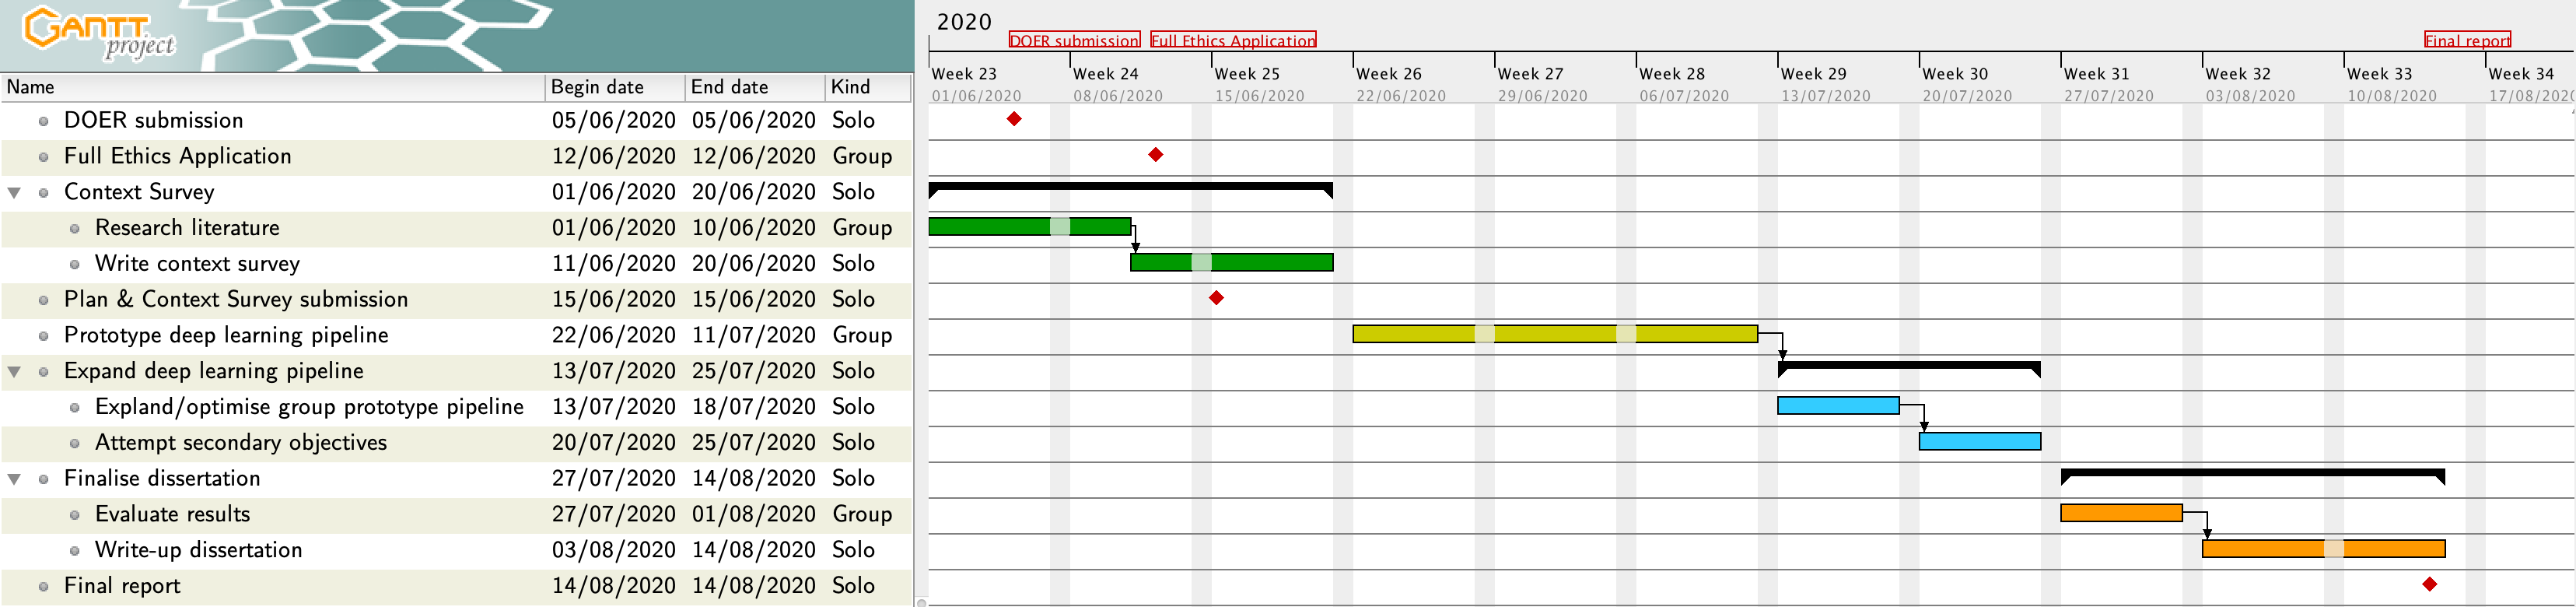
\includegraphics[width=\textwidth]{Plan & Draft Context Survey/figures/gantt_chart.png}}
\caption{\label{fig:gantt_chart}Gantt Chart ranging from 01/06/2020 to 14/08/2020.}
\end{figure}


% ------------------- Draft Context Survey --------------------

\section{Draft Context Survey}
\label{sec:draft-context-survey}

\subsection{Breast Cancer Detection}

\subsubsection{The History of Breast Cancer Detection}

The detection of breast cancer using mammograms, and any form of cancer using medical imagery, relies on the conventional diagnoses of expert radiologists \cite{Osareh2010}. These diagnoses rest on the correct interpretation of the mammograms, which may be subject to errors due to the difficulty of correctly interpreting them \cite{Elter2009}. To assist radiologists in their interpretation, Computer-Assisted Detection/Diagnosis (CAD) software 

\subsubsection{Motivation of Using Deep Learning Systems in Breast Cancer Detection}

History of breast cancer detection (leads to)\\
Motivation of using ML/DL for breast detection\\
Problems with current breast cancer detection systems

\subsection{Deep Learning applications to breast cancer detection}
Other work done in this subject (and their results/observations)\\
Naturally lead towards deep neural networks (e.g. CNNs) for part 3

\subsection{Deep Learning techniques \& Convolutional Neural Networks}
Explore the techniques used in deep learning (techniques, databases, processing, libraries, output metrics, etc.)\\
Explore the deep learning model that will be explored by each dissertation

% -------------------- APPENDIX --------------------

\begin{appendices}

\clearpage
\bibliographystyle{unsrt}
\bibliography{BibliographyPlan}

\end{appendices}
\end{document}